\section{Five-Agent Architecture}
\label{sec:concept-architecture}

The modular architecture of \textit{Invox} is organized into five specialized agents. Each agent exposes a clear input/output contract, enabling component-level analysis, flexible substitution, and isolated improvement. This section characterizes the roles of the agents and their interconnections, independent of any particular deployment strategy.

\begin{figure}[H]
  \centering
  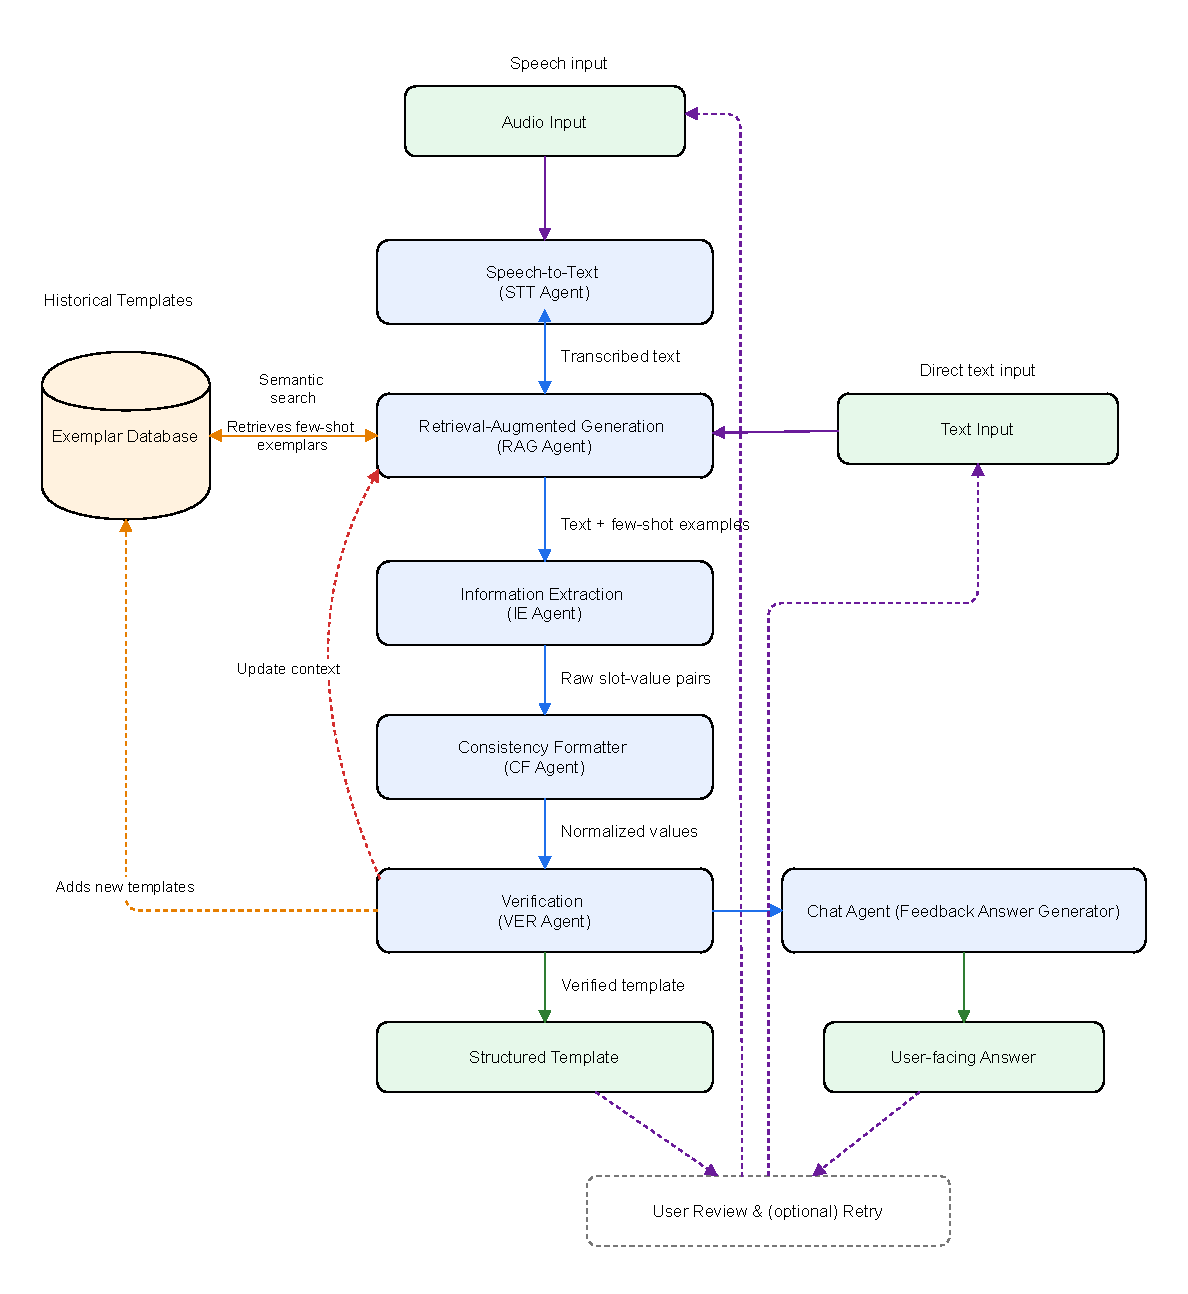
\includegraphics[width=1.0\linewidth]{images/agent_pipeline.drawio.pdf}
  \caption{Invox’s Five-Agent Pipeline}
  \label{fig:agent-pipeline}
\end{figure}



\subsection{Speech-to-Text Agent (STT)}
\label{subsec:stt-agent}

The STT agent converts spoken language into text using a Whisper-based transcription model \cite{radford2023whisper}. It accepts audio recordings as input and outputs transcribed text along with metadata such as word-level confidence scores, timestamps, and language detection results. As the focus of this work is the mapping from unstructured text to template fields, the STT component remains an adapter rather than the core of the architecture. Textual inputs bypass this stage and enter directly into the RAG agent.

\textbf{Design considerations.} The STT agent is deliberately shallow to maintain generality. Whisper was selected for its robustness to noise and multilingual support, which are critical in industrial environments where background machinery, accents, and code-switching are common \cite{fathullah2023prompting}. Alternative ASR systems could be substituted without affecting downstream components, provided they produce UTF-8 text output.

\subsection{Retrieval-Augmented Generation Agent (RAG)}
\label{subsec:rag-agent}

The RAG agent enhances extraction accuracy by retrieving relevant examples from historical data before template filling begins. It accepts the transcribed or typed text as input and queries an indexed corpus—comprising previously completed templates—using semantic similarity search over dense vector embeddings. The agent outputs the top-$k$ most relevant examples, which are passed alongside the user input to the IE agent as few-shot context.

\textbf{Retrieval mechanism.} The RAG agent encodes input text using a pretrained sentence transformer and performs cosine similarity search against stored template embeddings. The system returns $k$ ranked examples (typically $k = 3$–$5$), each containing the original text and its corresponding template completion.

\textbf{Design rationale.} This agent directly addresses R2 (information extraction) and R5 (learning and adaptation). By dynamically selecting examples tailored to the current input, the system avoids the brittleness of static few-shot prompts while benefiting from organizational memory \cite{mialon2023augmented}. The semantic search ensures that examples are retrieved based on conceptual similarity, making the system robust to paraphrasing and vocabulary variations. Over time, as more templates are completed and added to the index, extraction accuracy improves without requiring model retraining.

\subsection{Information Extraction Agent (IE)}
\label{subsec:ie-agent}

The IE agent performs the central task of transforming unstructured text into structured template fields. Its input consists of three components: (1) the free-form text (transcribed or provided directly), (2) the retrieved few-shot examples from the RAG agent, and (3) the target template schema specifying which fields need to be filled. The agent outputs candidate slot-value pairs for all specified fields in the template schema.

The agent operates by prompting a large language model with task-specific instructions and examples. For each field in the template schema, the model attempts to extract relevant information from the input text. If information for a particular field cannot be found in the text, the field is explicitly populated with a null value rather than being omitted. This ensures completeness while maintaining the structured output format.

\textbf{Processing approach:}
\begin{itemize}
    \item \textbf{Schema-driven extraction:} The agent processes all fields specified in the template schema, ensuring comprehensive coverage of the required information structure.
    \item \textbf{Evidence-based population:} Fields are populated only when supporting evidence is present in the input text, preventing hallucination of unsupported values.
    \item \textbf{Explicit null handling:} When information for a field is unavailable in the text, the field is explicitly marked as null, maintaining the complete output structure.
\end{itemize}

\textbf{Prompt structure.} The IE agent's prompt consists of four components: (1) task definition specifying the target schema and fields, (2) retrieved few-shot examples demonstrating successful extraction patterns, (3) the current user input text, and (4) output format constraints requiring JSON-structured responses that include all specified fields. This structure ensures consistent output formatting while leveraging the contextual understanding provided by few-shot examples \cite{zhang2023sgptod}.

\subsection{Consistency Formatting Agent (CF)}
\label{subsec:cf-agent}

The CF agent transforms the raw extracted values from the IE agent into standardized, schema-compliant formats. It accepts the slot-value pairs produced by the IE agent and applies deterministic normalization rules and schema validation to ensure consistency across all template outputs.

\textbf{Schema validation and normalization:}
\begin{itemize}
    \item \textbf{Data type enforcement:} Converts extracted values to appropriate data types (dates to ISO format, numbers to numerical types, etc.) and validates against schema constraints
    \item \textbf{Value canonicalization:} Standardizes variations using deterministic rules (e.g., ``Sept. 11'' → ``2001-09-11'', ``USA'' → ``United States'')
    \item \textbf{Controlled vocabulary mapping:} Enforces domain-specific conventions by mapping extracted terms to predefined categories for incident types, equipment codes, and other standardized fields
    \item \textbf{Schema compliance checking:} Validates that all values conform to the template schema requirements, including format constraints and value ranges
\end{itemize}

\textbf{Normalization approach.} The CF agent employs both deterministic transformations and LLM-based resolution for ambiguous cases. Structured data types like dates, numbers, and standard identifiers are normalized using regular expressions and parsing libraries. For ambiguous entities—such as informal location names or context-dependent equipment codes—the agent can prompt an LLM with the original context and domain glossaries to resolve variations. This hybrid approach balances precision with contextual awareness while maintaining deterministic behavior for well-defined formats.

\textbf{Design rationale.} By separating normalization from extraction, the system ensures consistent output formatting regardless of input variations while enforcing schema compliance. This addresses requirement R1 (consistency) and allows the IE agent to focus solely on content identification rather than format enforcement \cite{gatt2018survey}. The CF agent also reduces evaluation noise by ensuring that performance comparisons across different extraction strategies are not confounded by formatting inconsistencies.

\subsection{Verification Agent (VER)}
\label{subsec:ver-agent}

The VER agent performs comprehensive quality assessment on the structured template produced by the CF agent. It accepts the normalized slot-value pairs as input and generates a fully verified template with confidence scoring, field-level annotations, and interactive clarification capabilities.

\textbf{Quality assessment components:}
\begin{itemize}
    \item \textbf{Confidence scoring:} Assigns confidence scores to each populated field based on extraction quality, evidence strength, and internal consistency metrics
    \item \textbf{Field annotations:} Provides detailed annotations for each field indicating the source evidence, extraction method, and any processing notes
    \item \textbf{Conflict detection:} Identifies internal contradictions or inconsistencies between related fields (e.g., conflicting dates, incompatible equipment types)
    \item \textbf{Completeness validation:} Flags required fields that remain empty or contain insufficient information
\end{itemize}

\textbf{Interactive clarification system.} When low-confidence fields, conflicts, or missing required information are detected, the VER agent generates targeted chat messages to solicit user clarification. These messages are context-aware and focus specifically on the uncertain aspects of the template, enabling iterative refinement through user feedback. The system maintains conversation history to provide context for subsequent clarification rounds.

\textbf{Final output generation.} The VER agent produces the completed template with all quality annotations, making transparent which fields are highly reliable versus those requiring user verification. This includes:
\begin{itemize}
    \item Confidence scores for automated quality assessment
    \item Evidence references linking extracted values to source text spans
    \item Clear indicators of fields that may need user attention
    \item Structured data ready for database integration or further processing
\end{itemize}

\textbf{Design rationale.} VER directly supports R3 (transparency) by providing comprehensive field-level annotations and confidence metrics, and R4 (user correction) through its interactive clarification system. By centralizing quality assessment and user interaction in a dedicated agent, the system ensures consistent verification standards while maintaining clear separation from the extraction and normalization processes \cite{park2023generative}.

\subsection{Agent Interfaces and Data Flow}
\label{subsec:agent-interfaces}

Table~\ref{tab:agent-interfaces} summarizes the interface of each agent. By separating their responsibilities and outputs, the architecture supports substitution of different models, logging of intermediate states, and detailed error analysis. Figure~\ref{fig:agent-pipeline-enhanced} illustrates the sequential data flow through the five agents for both audio and text inputs.

\begin{table}[h]
\centering
\begin{tabular}{p{2.5cm}p{5cm}p{5.5cm}}
\toprule
\textbf{Agent} & \textbf{Input} & \textbf{Output} \\
\midrule
\textbf{STT} & Audio signal & Transcribed text with metadata (confidence scores, timestamps) \\
\midrule
\textbf{RAG} & Text (transcribed or direct input) & Top-$k$ retrieved examples with relevance scores and template mappings \\
\midrule
\textbf{IE} & Text + retrieved examples + template schema & Candidate slot-value pairs (null for unavailable fields) \\
\midrule
\textbf{CF} & Raw slot-value pairs & Normalized values with schema validation and format standardization \\
\midrule
\textbf{VER} & Normalized slot-value pairs & Verified template with confidence scores, field annotations, and clarification prompts \\
\bottomrule
\end{tabular}
\caption{Invox's Agent interfaces and data flow}
\label{tab:agent-interfaces}
\end{table}

The next section formalizes four deployment strategies that instantiate this architecture with different orchestration patterns, trading off accuracy, latency, and computational cost.

